\par Dark current is a very large limiting factor in the performance of an image sensor. Image sensors work by generating a signal when an area of the signal has a different light level than the rest and it is able to then generate a pixel. Dark currents "occur in every pixel, but vary from pixel-to-pixel" based on a number of factors such as heat on the image sensor. Due to how pervasive dark currents are for image sensors there is a lot of research going into how to possibly prevent any dark currents. Over the past 40 years there has been nearly a large (5500x) drop in the dark current for image sensors, however this is still too high for many applications of image sensors\cite{mcgrath_tobin_goiffon_magan_2018}.
\begin{figure}[H]
    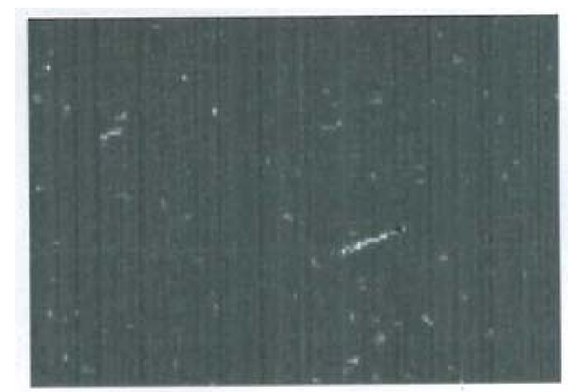
\includegraphics[width=\linewidth]{json star tracker}
    \caption{JSON 1 Star Tracker Source:\cite{bardoux_penquer_gilard_ecoffet_auvergne_2017}}
    \label{fig:startracker}
\end{figure}
\par Star trackers on satellites need incredibly precise images to accurately calculate the vehicle position. Star trackers work by taking images and calculating their position based on the location of known stars. Any noise or dark currents induced in these sensors can result in large miscalculations. \autoref{fig:startracker} is an image taken from the JNSON 1 satellite star tracker. This image is significant because it shows how there is so much noise in this critical system. If the algorithm for calculating the position of the satellite has too many false positives due to dark currents the satellite can shut down and go into a "survival" configuration until the situation can be resolved \cite{bardoux_penquer_gilard_ecoffet_auvergne_2017}. This would prevent the satellite's mission from being continued until it can recalculate its location. In cases like star trackers on satellites dark current is a very dangerous fault and motivates research into various solutions to dark currents in CMOS sensors.